% YOLO11n as a ladder: backbone on top, neck under it, heads at the bottom, aligned by scale.
% Boxes use the PlotNeuralNet layer (MIT). Size follows the feature map, thickness follows the channels.
\documentclass[border=5pt, tikz]{standalone}
\usepackage{newtxtext,newtxmath}
\usepackage{import}
\subimport{pnn/}{init}
\usetikzlibrary{positioning,calc,arrows.meta}
\definecolor{sbblue}{RGB}{20,60,200}
\definecolor{sbgreen}{RGB}{120,180,20}
\definecolor{sbred}{RGB}{200,30,30}
\definecolor{ink}{RGB}{40,40,40}
\def\Bb{sbblue!30}\def\Nk{sbgreen!35}\def\Hd{sbred!50}
% \fm{name}{x}{y}{fill}{size}{thickness}{label}: thickness and size in PlotNeuralNet units
\newcommand{\fm}[7]{%
  \pgfmathsetmacro{\halfw}{#6*0.1}%
  \pgfmathsetmacro{\dep}{#5*0.6}%
  \pic[shift={(-\halfw,0,0)}] at (#2,#3) {Box={name=#1, caption=, zlabel=, fill=#4, height=#5, width=#6, depth=\dep}};
  \pgfmathsetmacro{\lift}{\dep*0.2*0.5*0.385+0.1}%
  \node[anchor=south west, font=\footnotesize, text=ink, inner sep=1pt] at ($(#1-north)+(0.1,\lift)$) {#7};}
\newcommand{\merge}[3]{\pic at (#2,#3) {Ball={name=#1, fill=white, radius=1.3, logo=$\|$}};}
\begin{document}
\begin{tikzpicture}[font=\small]
\tikzstyle{flow}=[line width=1.3pt, draw=ink, -{Stealth[length=2.6mm]}]
\tikzstyle{elbow}=[flow, rounded corners=4pt]
\def\cA{1.2}\def\cB{3.7}\def\cC{6.4}\def\cD{9.6}\def\cE{12.8}\def\cF{15.4}
\def\rB{0}\def\rM{-2.2}\def\rT{-3.5}\def\rN{-5.0}\def\rU{-6.3}\def\rH{-8.4}

% input
\node[inner sep=0] (img) at (-1.0,\rB) {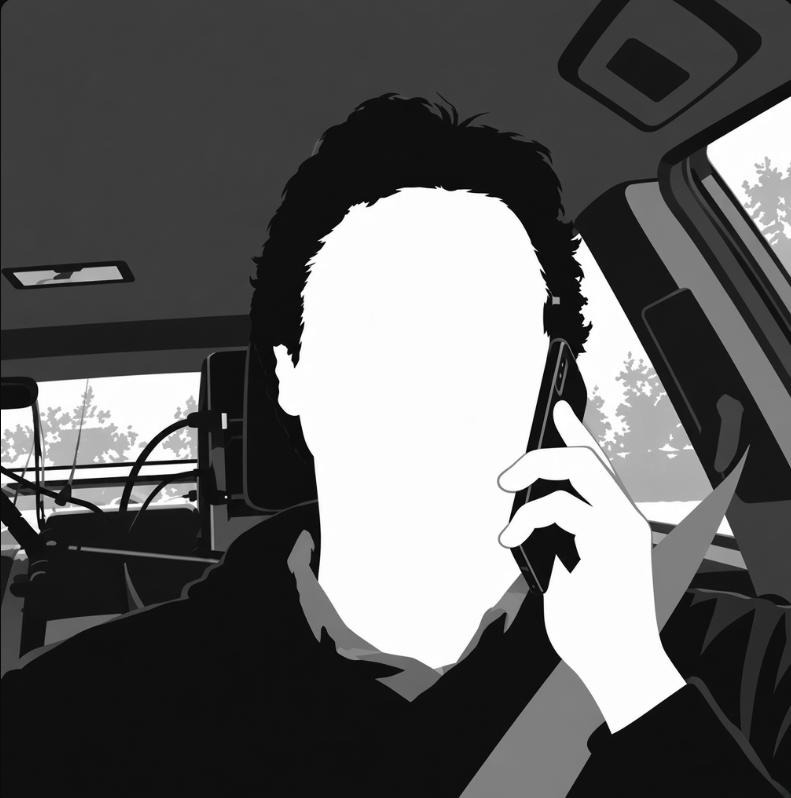
\includegraphics[width=2.1cm]{../../Figures/guide_1.png}};
\node[anchor=north, font=\footnotesize, text=ink] at (img.south) {640$\times$640};

% backbone: 320 to 20
\fm{b1}{\cA}{\rB}{\Bb}{14}{1}{320}
\fm{b2}{\cB}{\rB}{\Bb}{11}{2}{160}
\fm{b3}{\cC}{\rB}{\Bb}{8.5}{3}{80}
\fm{b4}{\cD}{\rB}{\Bb}{6.5}{3}{40}
\fm{b5}{\cE}{\rB}{\Bb}{4.5}{4}{20}
\fm{sp}{\cF}{\rB}{sbblue!55}{4.5}{4}{SPPF, C2PSA}
\draw[flow] (img.east) -- (b1-west);
\foreach \a/\b in {b1/b2,b2/b3,b3/b4,b4/b5,b5/sp} \draw[flow] (\a-east) -- (\b-west);

% neck, top-down: merge with the backbone at 40, then at 80
\merge{m4}{\cD}{\rM}
\merge{m3}{\cC}{\rM}
\fm{t4}{\cD}{\rT}{\Nk}{6.5}{3}{}
\fm{t3}{\cC}{\rT}{\Nk}{8.5}{2}{}
\draw[flow] (b4-south) -- (m4-north);
\draw[flow] (b3-south) -- (m3-north);
\draw[elbow] (sp-south) |- node[pos=0.75, above, font=\footnotesize, text=gray]{$\times 2$} (m4-east);
\draw[flow] (m4-south) -- (t4-north);
\draw[flow] (m3-south) -- (t3-north);
\draw[elbow] (t4-west) -- ++(-0.75,0) |- node[pos=0.72, above, font=\footnotesize, text=gray]{$\times 2$} (m3-east);

% neck, bottom-up: merge back at 40, then at 20
\merge{n4}{\cD}{\rN}
\merge{n5}{\cE}{\rN}
\fm{u3}{\cC}{\rU}{\Nk}{8.5}{2}{}
\fm{u4}{\cD}{\rU}{\Nk}{6.5}{3}{}
\fm{u5}{\cE}{\rU}{\Nk}{4.5}{4}{}
\draw[flow] (t3-south) -- (u3-north);
\draw[flow] (t4-south) -- (n4-north);
\draw[elbow] (u3-east) -- ++(0.75,0) |- node[pos=0.72, above, font=\footnotesize, text=gray]{$\div 2$} (n4-west);
\draw[flow] (n4-south) -- (u4-north);
\draw[elbow] (u4-east) -- ++(0.75,0) |- node[pos=0.72, above, font=\footnotesize, text=gray]{$\div 2$} (n5-west);
\draw[flow] (n5-south) -- (u5-north);
\draw[elbow] (sp-south) |- (n5-east);

% heads: one per scale
\foreach \n/\x/\s/\t in {3/\cC/5/small cues (80), 4/\cD/4/medium (40), 5/\cE/3/large (20)} {
  \pic[shift={(-0.12,0,0)}] at (\x,\rH) {Box={name=h\n, caption=, zlabel=, fill=\Hd, height=\s, width=1.2, depth=\s*0.6}};
  \draw[flow] (u\n-south) -- (h\n-north);
  \node[anchor=north, font=\footnotesize, text=ink] at ($(h\n-south)+(0,-0.2)$) {\t};
}
\node[anchor=west, align=left, font=\footnotesize, text=ink] (out) at (\cF-0.75,\rH) {NMS, then box,\\class, score};
\draw[flow] (h5-east) -- (out.west);

% group names on the left, one per row
\node[anchor=west, text=sbblue, font=\normalsize\bfseries] at (-2.05,-1.75) {Backbone};
\node[anchor=west, text=sbgreen!65!black, font=\normalsize\bfseries] at (-2.05,-4.9) {Neck};
\node[anchor=west, text=sbred, font=\normalsize\bfseries] at (-2.05,\rH) {Heads};
\end{tikzpicture}
\end{document}
